\documentclass[11pt,a4paper]{report}
\usepackage[textwidth=37em,vmargin=30mm]{geometry}
\usepackage{calc,xunicode,amsmath,amssymb,paralist,enumitem,tabu,booktabs,datetime2,xeCJK,xeCJKfntef,listings}
\usepackage{tocloft,fancyhdr,tcolorbox,xcolor,graphicx,eso-pic,xltxtra,xelatexemoji}

\newcommand{\envyear}[0]{2025}
\newcommand{\envdatestr}[0]{2025-08-31}
\newcommand{\envfinaldir}[0]{webdb/2025/20250831/final}

\usepackage[hidelinks]{hyperref}
\hypersetup{
    colorlinks=false,
    pdfpagemode=FullScreen,
    pdftitle={Web Digest - \envdatestr}
}

\setlength{\cftbeforechapskip}{10pt}
\renewcommand{\cftchapfont}{\rmfamily\bfseries\large\raggedright}
\setlength{\cftbeforesecskip}{2pt}
\renewcommand{\cftsecfont}{\sffamily\small\raggedright}

\setdefaultleftmargin{2em}{2em}{1em}{1em}{1em}{1em}

\usepackage{xeCJK,xeCJKfntef}
\xeCJKsetup{PunctStyle=plain,RubberPunctSkip=false,CJKglue=\strut\hskip 0pt plus 0.1em minus 0.05em,CJKecglue=\strut\hskip 0.22em plus 0.2em}
\XeTeXlinebreaklocale "zh"
\XeTeXlinebreakskip = 0pt


\setmainfont{Brygada 1918}
\setromanfont{Brygada 1918}
\setsansfont{IBM Plex Sans}
\setmonofont{JetBrains Mono NL}
\setCJKmainfont{Noto Serif CJK SC}
\setCJKromanfont{Noto Serif CJK SC}
\setCJKsansfont{Noto Sans CJK SC}
\setCJKmonofont{Noto Sans CJK SC}

\setlength{\parindent}{0pt}
\setlength{\parskip}{8pt}
\linespread{1.15}

\lstset{
	basicstyle=\ttfamily\footnotesize,
	numbersep=5pt,
	backgroundcolor=\color{black!5},
	showspaces=false,
	showstringspaces=false,
	showtabs=false,
	tabsize=2,
	captionpos=b,
	breaklines=true,
	breakatwhitespace=true,
	breakautoindent=true,
	linewidth=\textwidth
}






\newcommand{\coverpic}[2]{
    % argv: itemurl, authorname
    Cover photo by #2~~(\href{#1}{#1})
}
\newcommand{\makeheader}[0]{
    \begin{titlepage}
        % \newgeometry{hmargin=15mm,tmargin=21mm,bmargin=12mm}
        \begin{center}
            
            \rmfamily\scshape
            \fontspec{BaskervilleF}
            \fontspec{Old Standard}
            \fontsize{59pt}{70pt}\selectfont
            WEB\hfill DIGEST
            
            \vfill
            % \vskip 30pt
            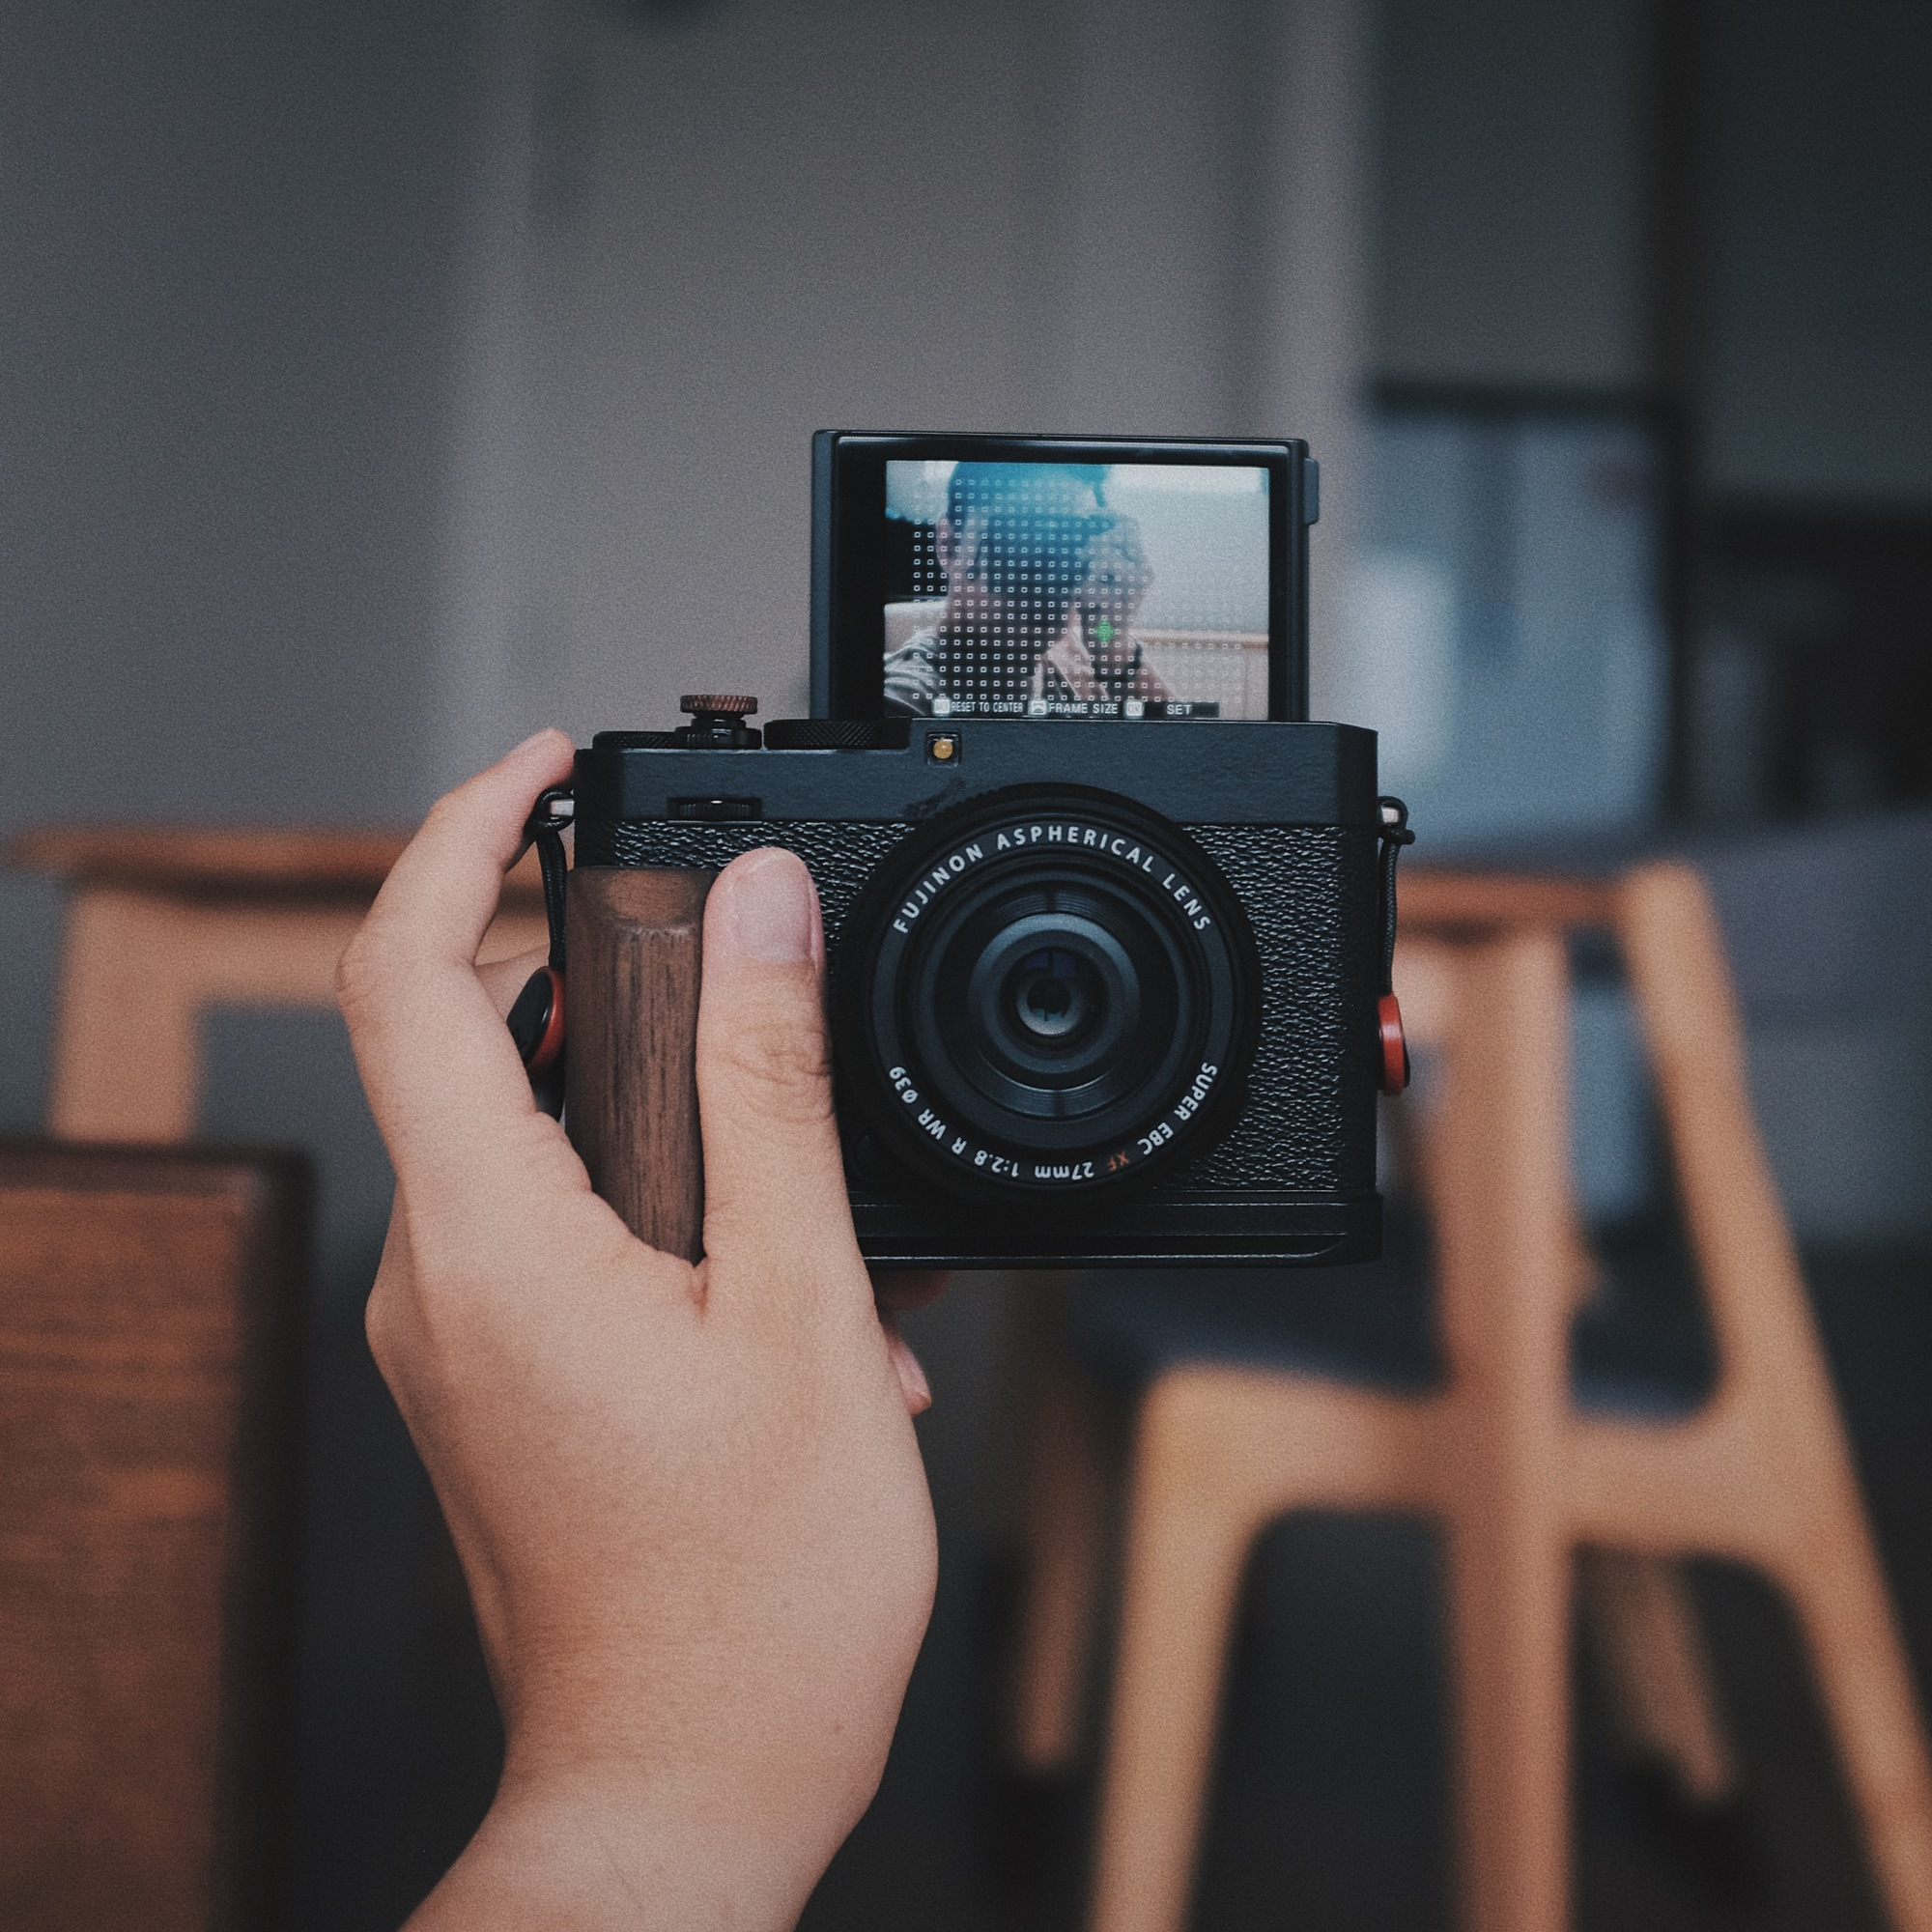
\includegraphics[width=\linewidth]{\envfinaldir/coverpic-prod.jpg}\par
            % \vskip 30pt
            \vfill

            \normalsize\rmfamily\scshape
            \copyright{} The Web Digest Project \hfill\large \envdatestr
        \end{center}
    \end{titlepage}
    % \restoregeometry
}
\newcommand{\simplehref}[1]{%
    \textcolor{blue!80!green}{\href{#1}{#1}}%
}
\renewcommand{\contentsname}{\center\Huge\sffamily\bfseries Contents\par\vskip 20pt}
\newcounter{ipartcounter}
\setcounter{ipartcounter}{0}
\newcommand{\ipart}[1]{
    % \vskip 20pt
    \clearpage
    \stepcounter{ipartcounter}
    \phantomsection
    \addcontentsline{toc}{chapter}{#1}
    % \begin{center}
    %     \Huge
    %     \sffamily\bfseries
    %     #1
    % \end{center}
    % \vskip 20pt plus 7pt
}
\newcounter{ichaptercounter}
\setcounter{ichaptercounter}{0}
\newcommand{\ichapter}[1]{
    % \vskip 20pt
    \clearpage
    \stepcounter{ichaptercounter}
    \phantomsection
    \addcontentsline{toc}{section}{\numberline{\arabic{ichaptercounter}}#1}
    \begin{center}
        \Huge
        \sffamily\bfseries
        #1
    \end{center}
    \vskip 20pt plus 7pt
}
\newcommand{\entrytitlefont}[1]{\subsection*{\raggedright\Large\sffamily\bfseries#1}}
\newcommand{\entryitemGeneric}[2]{
    % argv: title, url
    \parbox{\linewidth}{
        \entrytitlefont{#1}\par\vskip 5pt
        \footnotesize\ttfamily\mdseries
        \simplehref{#2}
    }\vskip 11pt plus 11pt minus 1pt
}
\newcommand{\entryitemGithub}[3]{
    % argv: title, url, desc
    \parbox{\linewidth}{
        \entrytitlefont{#1}\par\vskip 5pt
        \footnotesize\ttfamily\mdseries
        \simplehref{#2}\par\vskip 5pt
        \small\rmfamily\mdseries#3
    }\vskip 11pt plus 11pt minus 1pt
}
\newcommand{\entryitemAp}[3]{
    % argv: title, url, desc
    \parbox{\linewidth}{
        \entrytitlefont{#1}\par\vskip 5pt
        \footnotesize\ttfamily\mdseries
        \simplehref{#2}\par\vskip 5pt
        \small\rmfamily\mdseries#3
    }\vskip 11pt plus 11pt minus 1pt
}
\newcommand{\entryitemHackernews}[3]{
    % argv: title, hnurl, rawurl
    % \parbox{\linewidth}{
    %     \entrytitlefont{#1}\par\vskip 5pt
    %     \footnotesize\ttfamily\mdseries
    %     \simplehref{#3}\par
    %     \textcolor{black!50}{\href{#2}{#2}}
    % }\vskip 11pt plus 11pt minus 1pt
    \begin{minipage}{\linewidth}
            \entrytitlefont{#1}\par\vskip 5pt
            \footnotesize\ttfamily\mdseries
            \simplehref{#3}\par
            \textcolor{black!50}{\href{#2}{#2}}
    \end{minipage}\par\vskip 11pt plus 11pt minus 1pt
}







\begin{document}

\makeheader

\tableofcontents\clearpage




\ipart{Developers}
\ichapter{Hacker News}
\entryitemTwoLinks{Six Months into Tariffs, Businesses Have No Idea How to Price Anything}{https://news.ycombinator.com/item?id=45077937}{https://www.wsj.com/business/retail/trump-tariff-business-price-impact-37b630c8}

\entryitemTwoLinks{Are we decentralized yet?}{https://news.ycombinator.com/item?id=45077291}{https://arewedecentralizedyet.online/}

\entryitemTwoLinks{The Sex Recession: The Share of Americans Having Regular Sex Keeps Dropping}{https://news.ycombinator.com/item?id=45075699}{https://ifstudies.org/blog/the-sex-recession-the-share-of-americans-having-regular-sex-keeps-dropping}

\entryitemTwoLinks{You Have to Feel It}{https://news.ycombinator.com/item?id=45075048}{https://mitchellh.com/writing/feel-it}

\entryitemTwoLinks{Condor's Cuzco RISC-V Core at Hot Chips 2025}{https://news.ycombinator.com/item?id=45074895}{https://chipsandcheese.com/p/condors-cuzco-risc-v-core-at-hot}

\entryitemTwoLinks{AI models need a virtual machine}{https://news.ycombinator.com/item?id=45074467}{https://blog.sigplan.org/2025/08/29/ai-models-need-a-virtual-machine/}

\entryitemTwoLinks{Bcachefs Goes to "Externally Maintained"}{https://news.ycombinator.com/item?id=45074312}{https://lwn.net/Articles/1035736/}

\entryitemTwoLinks{Cognitive load is what matters}{https://news.ycombinator.com/item?id=45074248}{https://github.com/zakirullin/cognitive-load}

\entryitemTwoLinks{FBI cyber cop: Salt Typhoon pwned 'nearly every American'}{https://news.ycombinator.com/item?id=45074157}{https://www.theregister.com/2025/08/28/fbi\_cyber\_cop\_salt\_typhoon/}

\entryitemTwoLinks{Agent Client Protocol (ACP)}{https://news.ycombinator.com/item?id=45074147}{https://agentclientprotocol.com/overview/introduction}

\entryitemTwoLinks{Nokia's legendary font makes for a great user interface font}{https://news.ycombinator.com/item?id=45074071}{https://www.osnews.com/story/143222/it-turns-out-nokias-legendary-font-makes-for-a-great-general-user-interface-font/}

\entryitemTwoLinks{Hardening Firefox – a checklist for improved browser privacy}{https://news.ycombinator.com/item?id=45073746}{https://andrewmarder.net/firefox/}

\entryitemTwoLinks{From multi-head to latent attention: The evolution of attention mechanisms}{https://news.ycombinator.com/item?id=45072160}{https://vinithavn.medium.com/from-multi-head-to-latent-attention-the-evolution-of-attention-mechanisms-64e3c0505f24}

\entryitemTwoLinks{Show HN: Hacker News em dash user leaderboard pre-ChatGPT}{https://news.ycombinator.com/item?id=45071722}{https://www.gally.net/miscellaneous/hn-em-dash-user-leaderboard.html}

\entryitemTwoLinks{Pentagon Docs: US Wants to "Suppress Dissenting Arguments" Using AI Propaganda}{https://news.ycombinator.com/item?id=45071063}{https://theintercept.com/2025/08/25/pentagon-military-ai-propaganda-influence/}

\entryitemTwoLinks{Why Romania excels in international Olympiads}{https://news.ycombinator.com/item?id=45070793}{https://www.palladiummag.com/2025/08/29/why-romania-excels-in-international-olympiads/}

\entryitemTwoLinks{The Theoretical Limitations of Embedding-Based Retrieval}{https://news.ycombinator.com/item?id=45068986}{https://arxiv.org/abs/2508.21038}

\entryitemTwoLinks{How did .agakhan, .ismaili and .imamat get their own TLDs?}{https://news.ycombinator.com/item?id=45068215}{https://data.iana.org/TLD/tlds-alpha-by-domain.txt}

\entryitemTwoLinks{Do the simplest thing that could possibly work}{https://news.ycombinator.com/item?id=45068091}{https://www.seangoedecke.com/the-simplest-thing-that-could-possibly-work/}

\entryitemTwoLinks{Data engineering and software engineering are converging}{https://news.ycombinator.com/item?id=45067867}{https://clickhouse.com/blog/eight-principles-of-great-developer-experience-for-data-infrastructure}


\ipart{Developers~~~~(zh-Hans)}
\ichapter{Solidot}
\entryitemGeneric{\hskip 0pt{}为平衡能耗和生存演化可能对大脑大小设置了上限}{https://www.solidot.org/story?sid=82182}

\entryitemGeneric{\hskip 0pt{}超加工食品可能是男性精子质量下降的一个原因}{https://www.solidot.org/story?sid=82181}

\entryitemGeneric{\hskip 0pt{}Valve 为遵守法律对访问成人内容的英国用户验证年龄}{https://www.solidot.org/story?sid=82180}

\entryitemGeneric{\hskip 0pt{}银河麒麟发布 V11,安装量达到 1600 万}{https://www.solidot.org/story?sid=82179}

\entryitemGeneric{\hskip 0pt{}良品铺子的 AI 广告显示花生长在树上}{https://www.solidot.org/story?sid=82177}

\entryitemGeneric{\hskip 0pt{}年轻人没有以前快乐了}{https://www.solidot.org/story?sid=82176}

\entryitemGeneric{\hskip 0pt{}美国将限制留学生和记者签证有效期}{https://www.solidot.org/story?sid=82175}

\entryitemGeneric{\hskip 0pt{}黄石公园内自由迁徙的野牛加强了草原的恢复力}{https://www.solidot.org/story?sid=82174}

\entryitemGeneric{\hskip 0pt{}美商务部长称将在区块链上发布经济数据}{https://www.solidot.org/story?sid=82173}

\entryitemGeneric{\hskip 0pt{}日本小镇考虑倡导每天仅使用智能手机两小时}{https://www.solidot.org/story?sid=82172}

\entryitemGeneric{\hskip 0pt{}FFmpeg 8 支持实时生成字幕}{https://www.solidot.org/story?sid=82171}

\entryitemGeneric{\hskip 0pt{}研究显示 AI 的普及与美国初级工作的减少相关}{https://www.solidot.org/story?sid=82170}

\entryitemGeneric{\hskip 0pt{}美国共和党人调查维基百科的自由主义偏见}{https://www.solidot.org/story?sid=82169}

\entryitemGeneric{\hskip 0pt{}用流行病学分析法国大革命}{https://www.solidot.org/story?sid=82168}

\entryitemGeneric{\hskip 0pt{}开源项目通常由一个人维护}{https://www.solidot.org/story?sid=82167}

\entryitemGeneric{\hskip 0pt{}Nothing 成为最新一家被发现用图库照片演示手机摄影能力的厂商}{https://www.solidot.org/story?sid=82166}

\entryitemGeneric{\hskip 0pt{}源自 ChatGPT 的常用词在人们的日常对话中也日益流行}{https://www.solidot.org/story?sid=82165}

\entryitemGeneric{\hskip 0pt{}三名台积电工程师因窃取 2 纳米工艺机密被起诉}{https://www.solidot.org/story?sid=82164}

\entryitemGeneric{\hskip 0pt{}印度屏蔽 Sci-Hub}{https://www.solidot.org/story?sid=82163}

\entryitemGeneric{\hskip 0pt{}《K-POP:猎魔女团》成为 Netflix 史上观看次数最多的电影}{https://www.solidot.org/story?sid=82162}\ichapter{V2EX}
\entryitemGeneric{\hskip 0pt{}[分享创造] 开发了个 AI 编程开发者论坛, 欢迎大家使用}{https://www.v2ex.com/t/1156014}

\entryitemGeneric{\hskip 0pt{}[NAS] 给内网电脑开 SSH 的方案}{https://www.v2ex.com/t/1156013}

\entryitemGeneric{\hskip 0pt{}[奇思妙想] 大语言模型技术对人类社会产生的影响和改变}{https://www.v2ex.com/t/1156012}

\entryitemGeneric{\hskip 0pt{}[硬件] 最近选购 m2 无线网卡,同一个模块 jd 价格直接比 tb 翻倍,看评论销量还不少,求知欲一下子上来了想研究个明白}{https://www.v2ex.com/t/1156011}

\entryitemGeneric{\hskip 0pt{}[宽带症候群] 5GCPE 能获取到公网 ipv6 吗,入站有阻断吗}{https://www.v2ex.com/t/1156008}

\entryitemGeneric{\hskip 0pt{}[程序员] 尔智若神,何蠢如豕?平时人话都说不好,还指望 AI、vibe-coding?}{https://www.v2ex.com/t/1156006}

\entryitemGeneric{\hskip 0pt{}[创业组队] 金融量化项目寻找技术合伙人|全栈|北京}{https://www.v2ex.com/t/1156005}

\entryitemGeneric{\hskip 0pt{}[分享创造] 终于找到一个低成本使用 Nano Banana 的方案,顺便做了个网站}{https://www.v2ex.com/t/1156003}

\entryitemGeneric{\hskip 0pt{}[Claude] 听说 claude max 好多都死了,合租的大家有问题吗?}{https://www.v2ex.com/t/1156002}

\entryitemGeneric{\hskip 0pt{}[问与答] 请教一个关于 traccar 的问题}{https://www.v2ex.com/t/1156001}

\entryitemGeneric{\hskip 0pt{}[NAS] 黑群晖升级,这个 cpu 比蜗牛星际的 j9100 强吗}{https://www.v2ex.com/t/1156000}

\entryitemGeneric{\hskip 0pt{}[VPS] 有没有人出 dmit 的 hkg pro 套餐的老哥}{https://www.v2ex.com/t/1155999}

\entryitemGeneric{\hskip 0pt{}[职场话题] 在离职空档期,拿到一个着急入职的 offer 后又有面试电话,该不该面?}{https://www.v2ex.com/t/1155996}

\entryitemGeneric{\hskip 0pt{}[分享创造] WPS 的表格中插入的图片,在 Excel 中无法显示,在不安装 WPS 的情况下,有没有 macOS 上的转换工具?}{https://www.v2ex.com/t/1155995}

\entryitemGeneric{\hskip 0pt{}[程序员] openrouter 的免费 nano banana 模型}{https://www.v2ex.com/t/1155994}

\entryitemGeneric{\hskip 0pt{}[以太坊] 在家里跑 ETH、BSC 节点要紧不}{https://www.v2ex.com/t/1155992}

\entryitemGeneric{\hskip 0pt{}[南昌] 请问在 0791 地区的兄弟们,市区里哪里的小区板块值得入手。}{https://www.v2ex.com/t/1155991}

\entryitemGeneric{\hskip 0pt{}[硬件] [求助] 有无可以直接在 Windows 11 操作系统下虚拟出一个任意类型的 USB 设备的工具软件?}{https://www.v2ex.com/t/1155989}

\entryitemGeneric{\hskip 0pt{}[酷工作] [上海\&苏州]医药方向 AI Agent 公司 - 数据开发}{https://www.v2ex.com/t/1155987}

\entryitemGeneric{\hskip 0pt{}[程序员] 最近在多个渠道听到 Vibe Coding 这个概念,对于行业走向会产生什么影响}{https://www.v2ex.com/t/1155985}

\entryitemGeneric{\hskip 0pt{}[问与答] 长时间一个人在房间里呆着会影响精神状态,你们是怎么解决的}{https://www.v2ex.com/t/1155984}

\entryitemGeneric{\hskip 0pt{}[问与答] 有没有人知道 A 股里的涨跌停限制价格是如何计算出来的?}{https://www.v2ex.com/t/1155983}

\entryitemGeneric{\hskip 0pt{}[分享创造] VIVY - Stable Diffusion 桌面应用}{https://www.v2ex.com/t/1155981}

\entryitemGeneric{\hskip 0pt{}[macOS] 延续 macos 的意志,实现网页版的空格预览}{https://www.v2ex.com/t/1155980}

\entryitemGeneric{\hskip 0pt{}[酷工作] 需要部署基于 funasr 和 Paraformer 的语音识别接口,有没有大神可以支持}{https://www.v2ex.com/t/1155979}

\entryitemGeneric{\hskip 0pt{}[问与答] Windows 远程控制 Mac 电脑,有什么好软件吗?}{https://www.v2ex.com/t/1155978}

\entryitemGeneric{\hskip 0pt{}[Windows] 针对 windows 11 24H2 (KB5063878) 可能导致硬盘损坏的问题,现在微软提供了新的修复更新了吗?}{https://www.v2ex.com/t/1155977}

\entryitemGeneric{\hskip 0pt{}[程序员] 怎么获取 apple watch 监测的实时体征数据呢}{https://www.v2ex.com/t/1155976}

\entryitemGeneric{\hskip 0pt{}[Apple] 分享一个自用的 scriptable 小组件脚本,用于订阅 appstore 应用价格变化}{https://www.v2ex.com/t/1155975}

\entryitemGeneric{\hskip 0pt{}[分享创造] [免费功能] 一款可以一键分享你的代理和网站登录状态的工具}{https://www.v2ex.com/t/1155972}

\entryitemGeneric{\hskip 0pt{}[微信] 微信小程序的激励广告,收益如何呢?}{https://www.v2ex.com/t/1155970}

\entryitemGeneric{\hskip 0pt{}[程序员] 如何避免开发中常见模块的重复造轮子}{https://www.v2ex.com/t/1155969}

\entryitemGeneric{\hskip 0pt{}[Apple] [开源工具] 做了个 Launchpad 开源复刻,可迁移此前在 Launchpad 里的软件分组,为 macOS 26 做好准备}{https://www.v2ex.com/t/1155968}

\entryitemGeneric{\hskip 0pt{}[问与答] 玩 3A 游戏过程中切出去刷刷网页聊聊天,再切回去游戏会变卡,有解决办法么?}{https://www.v2ex.com/t/1155967}

\entryitemGeneric{\hskip 0pt{}[奇思妙想] 分享一个``完全自主研发''的``另类''词汇学习工具,支持学习任何语言的词汇}{https://www.v2ex.com/t/1155966}

\entryitemGeneric{\hskip 0pt{}[投资] 有用盈透的吗,听说关闭注册?}{https://www.v2ex.com/t/1155963}

\entryitemGeneric{\hskip 0pt{}[分享发现] 微信扫码在特定场景下会在用户无感知的情况下 bypass HTTPS 证书校验}{https://www.v2ex.com/t/1155962}

\entryitemGeneric{\hskip 0pt{}[问与答] 有没有看过橡果国际广告的,初中电视指南天天看}{https://www.v2ex.com/t/1155961}

\entryitemGeneric{\hskip 0pt{}[加密货币] 欧易 c2c 通过支付宝买币,试了 5 个都在付款时支付宝提示对方账户被风控无法转账。}{https://www.v2ex.com/t/1155960}

\entryitemGeneric{\hskip 0pt{}[海口] 动作人偶生成器}{https://www.v2ex.com/t/1155959}

\entryitemGeneric{\hskip 0pt{}[程序员] win11 锁屏后,不息屏}{https://www.v2ex.com/t/1155956}

\entryitemGeneric{\hskip 0pt{}[NAS] 零刻 ME mini 全闪 NAS``无 Wi-Fi 版''首销: N9516G+64G+1T}{https://www.v2ex.com/t/1155955}

\entryitemGeneric{\hskip 0pt{}[推广] Nano Banana AI Image Generator}{https://www.v2ex.com/t/1155954}

\entryitemGeneric{\hskip 0pt{}[游戏开发] 游戏开发图形化和脚本方式}{https://www.v2ex.com/t/1155953}

\entryitemGeneric{\hskip 0pt{}[分享创造] [免登录免注册] 纯好玩,一个 90\% 由 AI 构建的``玄学''网站}{https://www.v2ex.com/t/1155952}

\entryitemGeneric{\hskip 0pt{}[酷工作] 帮朋友找前端实习生,杭州滨江某大厂}{https://www.v2ex.com/t/1155951}

\entryitemGeneric{\hskip 0pt{}[随想] 说一说我对彩礼与嫁妆的看法}{https://www.v2ex.com/t/1155950}

\entryitemGeneric{\hskip 0pt{}[问与答] 网站内容监控系统求推荐}{https://www.v2ex.com/t/1155948}

\entryitemGeneric{\hskip 0pt{}[OpenWrt] 现在有能刷 openwrt 的 wifi 802.11be 亲民一些的家用路由器没?}{https://www.v2ex.com/t/1155947}

\entryitemGeneric{\hskip 0pt{}[问与答] 使用 whisper.cpp 加载 large-v3-turbo 模型生成字幕的问题}{https://www.v2ex.com/t/1155945}


\ipart{Generic News}







\clearpage
\leavevmode\vfill
\footnotesize

Copyright \copyright{} 2023-2025 Neruthes and other contributors.

This document is published with CC BY-NC-ND 4.0 license.

The entries listed in this newsletter may be copyrighted by their respective creators.

This newsletter is generated by the Web Digest project.

The newsletters are also delivered via Telegram channel \CJKunderline{\href{https://t.me/webdigestchannel}{https://t.me/webdigestchannel}}.\\
RSS feed is available at \CJKunderline{\href{https://webdigest.pages.dev/rss.xml}{https://webdigest.pages.dev/rss.xml}}.

This newsletter is available in PDF at
\CJKunderline{\href{https://webdigest.pages.dev/}{https://webdigest.pages.dev/}}.

The source code being used to generate this newsletter is available at\\
\CJKunderline{\href{https://github.com/neruthes/webdigest}{https://github.com/neruthes/webdigest}}.

This newsletter is also available in
\CJKunderline{\href{http://webdigest.pages.dev/readhtml/\envyear/WebDigest-20250831.html}{HTML}} and
\CJKunderline{\href{https://github.com/neruthes/webdigest/blob/master/markdown/\envyear/WebDigest-20250831.md}{Markdown}}.


\coverpic{https://unsplash.com/photos/mountains-illuminated-by-the-sun-with-the-moon-visible-0Iy940x8T1Y}{Marek Piwnicki}


\end{document}
